\chapter{PHÂN TÍCH VÀ THIẾT KẾ HỆ THỐNG}
\label{ch:chuong3}

\section{Phân tích yêu cầu hệ thống}
\label{sec:phan_tich_yeu_cau}

\subsection{Yêu cầu chức năng (Functional Requirements)}
Hệ thống SmartDorm được thiết kế nhằm đáp ứng đầy đủ các yêu cầu nghiệp vụ thực tiễn của ký túc xá đại học hiện đại:

\begin{enumerate}
    \item \textbf{Quản lý người dùng và Kiểm soát truy cập dựa trên vai trò (RBAC):}
    \begin{itemize}
        \item Hỗ trợ 3 nhóm vai trò phân quyền độc lập: \texttt{ADMIN} (Ban quản lý/Cán bộ kỹ thuật), \texttt{STUDENT} (Sinh viên nội trú), và \texttt{STAFF} (Nhân viên vận hành).
        \item Xác thực tài khoản an toàn thông qua JWT (JSON Web Tokens), mật khẩu được băm bằng thuật toán Bcrypt với hệ số Salt $10$.
        \item Quy trình đăng ký tài khoản sinh viên chuẩn hóa: Các trường bắt buộc gồm Họ tên, Mã số sinh viên (MSSV), Số điện thoại, Email định dạng tên miền trường học (\texttt{@student.edu.vn}). Tài khoản đăng ký mặc định nhận vai trò sinh viên, không được phép tự chọn vai trò quản trị viên.
    \end{itemize}

    \item \textbf{Quản lý danh mục Tòa nhà, Phòng ở và Giường nằm:}
    \begin{itemize}
        \item Quản lý thông tin phân cấp: Tòa nhà (Building) $\rightarrow$ Tầng (Floor) $\rightarrow$ Phòng (Room) $\rightarrow$ Giường nằm (Bed).
        \item Cho phép phân bổ sinh viên vào giường cụ thể trong phòng. Hệ thống tự động cập nhật sức chứa thực tế của phòng và hiển thị trạng thái phòng trên giao diện.
    \end{itemize}

    \item \textbf{Cơ chế sinh mã thẻ RFID tự động:}
    \begin{itemize}
        \item Khi sinh viên đăng ký tài khoản thành công và được phân bổ vào phòng ở cụ thể, hệ thống tự động kích hoạt thuật toán sinh mã định danh thẻ từ RFID duy nhất tương ứng với sinh viên đó (dựa trên chuỗi băm chuẩn hóa kết hợp giữa MSSV và mã phòng: $\text{UID} = \text{MD5}(\text{MSSV} + \text{RoomCode})[0:8]$).
        \item Dữ liệu thẻ được đồng bộ tức thời xuống thiết bị đầu đọc RC522 tại cửa phòng mà không đòi hỏi cán bộ quản lý phải thao tác cấu hình thủ công.
    \end{itemize}

    \item \textbf{Giám sát môi trường vi khí hậu và An toàn PCCC:}
    \begin{itemize}
        \item Thu thập liên tục các chỉ số: Nhiệt độ ($^\circ\text{C}$), Độ ẩm ($\%$) và Nồng độ khí gas/khói ($\%$) từ mỗi phòng gửi về định kỳ mỗi 5 giây qua MQTT.
        \item Tự động kích hoạt chuông còi báo động tại chỗ (Buzzer) và gửi cảnh báo khẩn cấp (Emergency Alert) lên máy chủ khi nồng độ gas $\ge 60\%$.
        \item Kích hoạt cơ chế an toàn PCCC nghiêm ngặt: Tự động ngắt toàn bộ relay điện sinh hoạt trong phòng khi nồng độ gas $\ge 80\%$ để ngăn chặn triệt để nguy cơ tia lửa điện phát sinh gây nổ.
    \end{itemize}

    \item \textbf{Điều khiển thiết bị và Khả năng Hoàn tác lệnh (Command with Undo):}
    \begin{itemize}
        \item Cho phép người dùng bật/tắt thiết bị đèn chiếu sáng, quạt thông gió, máy điều hòa và mở khóa cửa từ xa qua giao diện web.
        \item Lưu trữ toàn bộ lịch sử thao tác vào bảng \texttt{CommandHistory}, cho phép người quản trị hoàn tác lệnh gần nhất (Undo Last Command) để khôi phục trạng thái hoạt động trước đó của thiết bị.
    \end{itemize}

    \item \textbf{Dự báo phụ tải năng lượng và Phát hiện bất thường Trí tuệ nhân tạo:}
    \begin{itemize}
        \item Tự động trích xuất chuỗi đặc trưng thời gian và vi khí hậu để dự báo nhu cầu tiêu thụ điện trong 24 giờ tiếp theo bằng mô hình Gradient Boosting Huber Loss.
        \item Giám sát và phát hiện sớm các dấu hiệu tiêu thụ điện bất thường (thiết bị rò điện, chạy quá tải) bằng mô hình Isolation Forest.
        \item Cung cấp trợ lý ảo thông minh AI Copilot trả lời các câu hỏi truy vấn dữ liệu phòng của sinh viên và cán bộ quản lý.
    \end{itemize}
\end{enumerate}

\subsection{Yêu cầu phi chức năng (Non-Functional Requirements)}
\begin{itemize}
    \item \textbf{Độ trễ truyền nhận (Latency):} Độ trễ truyền gói tin từ lúc cảm biến phát hiện đến khi hiển thị trên giao diện web phải đạt dưới $50\text{ms}$ qua MQTT và dưới $20\text{ms}$ qua WebSockets. Thời gian đáp ứng của API điều khiển không vượt quá $200\text{ms}$.
    \item \textbf{Độ tin cậy và Tính sẵn sàng (Reliability \& Availability):} Hệ thống đảm bảo tính liên tục đạt $99.9\%$. Giao thức MQTT sử dụng QoS 1 đảm bảo không thất lạc các bản tin cảnh báo khẩn cấp.
    \item \textbf{An toàn điện trường học (Electrical Safety):} Nhằm triệt tiêu mọi rủi ro giật điện hoặc đoản mạch trong môi trường ký túc xá, hệ thống áp dụng phương pháp mô phỏng số thông minh (Digital Proxy) để giám sát và ước tính điện năng gián tiếp dựa trên trạng thái thiết bị và vi khí hậu, tuyệt đối không đấu nối các module đo điện áp lưới 220V trực tiếp (PZEM-004T) vào mạch vi điều khiển của sinh viên.
    \item \textbf{Tính mở rộng (Scalability):} Kiến trúc phân tầng và cơ sở dữ liệu TimescaleDB cho phép mở rộng giám sát từ 1 phòng thí nghiệm lên tới hàng trăm phòng ở trong toàn trường mà không làm suy giảm hiệu năng hệ thống.
\end{itemize}

\section{Kiến trúc tổng thể hệ thống 5 tầng}
\label{sec:kien_truc_tong_the}

Hệ thống SmartDorm được tổ chức theo kiến trúc 5 tầng phân tán, đảm bảo tính mô-đun hóa cao, dễ dàng bảo trì và mở rộng trong tương lai (xem Hình~\ref{fig:smartdorm_5layer_arch}).

\begin{figure}[H]
    \centering
    \begin{tikzpicture}[node distance=1.5cm, auto, >=stealth]
        \tikzstyle{layer} = [rectangle, draw=blue!80, fill=blue!5, text width=13.5cm, rounded corners, minimum height=1.4cm, font=\small]
        
        \node [layer, fill=teal!10, draw=teal!80] (l5) {
            \textbf{TẦNG 5: TRÌNH DIỄN VÀ QUẢN TRỊ NGHIỆP VỤ (Next.js 16 App Router)}\\
            $\bullet$ Phân hệ Admin Portal (Dashboard, Quản lý phòng, Điều khiển, Năng lượng, Cảnh báo PCCC, AI Center)\\
            $\bullet$ Phân hệ Student Portal (Cá nhân hóa phòng, Điều khiển thiết bị, Nhật ký ra vào, Hồ sơ cá nhân)
        };
        
        \node [layer, below of=l5, yshift=-0.5cm, fill=purple!10, draw=purple!80] (l4) {
            \textbf{TẦNG 4: TRÍ TUỆ NHÂN TẠO \& SUY LUẬN DỮ LIỆU (FastAPI Microservice)}\\
            $\bullet$ Mô hình Gradient Boosting Regressor (Huber Loss) $\rightarrow$ Dự báo phụ tải điện 24h ($R^2=0.9607$)\\
            $\bullet$ Mô hình Isolation Forest $\rightarrow$ Phát hiện bất thường thiết bị | Trợ lý ảo AI Copilot Assistant
        };
        
        \node [layer, below of=l4, yshift=-0.5cm, fill=blue!15, draw=blue!80] (l3) {
            \textbf{TẦNG 3: MÁY CHỦ TRUNG TÂM VÀ LƯU TRỮ DỮ LIỆU (NestJS + TimescaleDB)}\\
            $\bullet$ NestJS Core (RBAC, JWT, Observer Pattern, Strategy Alert, Command Pattern with Undo, Rule Engine)\\
            $\bullet$ Prisma ORM với 12 bảng thực thể | PostgreSQL tích hợp TimescaleDB Hypertables chuỗi thời gian
        };
        
        \node [layer, below of=l3, yshift=-0.5cm, fill=orange!10, draw=orange!80] (l2) {
            \textbf{TẦNG 2: MẠNG TRUYỀN THÔNG VÀ ĐIỀU PHỐI TIN NHẮN (MQTT Broker \& WebSockets)}\\
            $\bullet$ Eclipse Mosquitto MQTT Broker (Cổng 1883/8883, QoS 1, Keep-Alive, LWT)\\
            $\bullet$ Socket.io WebSocket Gateway (Cổng 3001, luồng dữ liệu thời gian thực hai chiều)
        };
        
        \node [layer, below of=l2, yshift=-0.5cm, fill=green!10, draw=green!80] (l1) {
            \textbf{TẦNG 1: THIẾT BỊ PHẦN CỨNG NHÚNG VÀ CẢM BIẾN (ESP32 DevKit V1 Edge Node)}\\
            $\bullet$ Thu thập: DHT22 (Nhiệt/Ẩm - GPIO 4), MQ-2 (Gas/Khói - GPIO 34 ADC), RFID RC522 (13.56MHz SPI)\\
            $\bullet$ Chấp hành: Relay 4 kênh cách ly quang (GPIO 25, 14, 12, 13), Còi Buzzer (GPIO 15), 4 Nút bấm
        };
        
        \draw [<->, line width=1.5pt] (l1) -- (l2);
        \draw [<->, line width=1.5pt] (l2) -- (l3);
        \draw [<->, line width=1.5pt] (l3) -- (l4);
        \draw [<->, line width=1.5pt] (l3) -- (l5);
    \end{tikzpicture}
    \caption{Kiến trúc tổng thể 5 tầng của Hệ thống KTX Thông minh SmartDorm}
    \label{fig:smartdorm_5layer_arch}
\end{figure}

\section{Thiết kế phần cứng và Sơ đồ nguyên lý mạch}
\label{sec:thiet_ke_phan_cung}

\subsection{Sơ đồ mạch mô phỏng thiết kế hệ thống trên Wokwi}
Mô hình phần cứng điều khiển phòng ký túc xá được thiết kế và mô phỏng hoàn chỉnh trên môi trường Wokwi Simulator với các linh kiện chuẩn xác theo đúng cấu hình hệ thống thực tế (xem Hình~\ref{fig:wokwi_circuit}).

\begin{figure}[H]
    \centering
    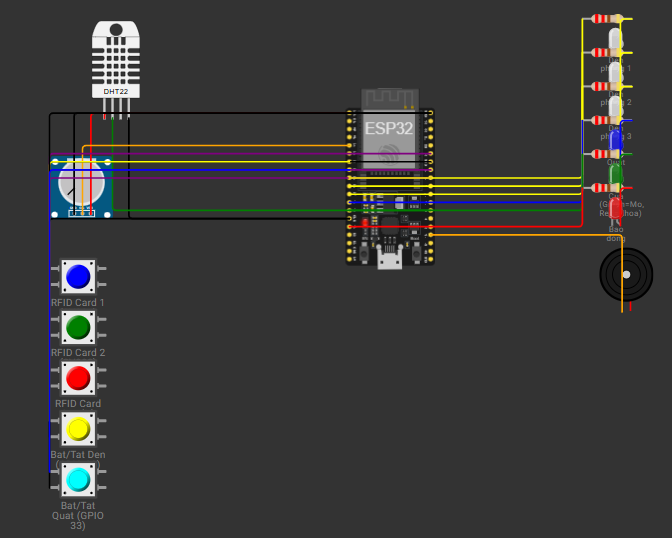
\includegraphics[width=0.88\textwidth]{figures/so_do_mach_mo_phong_wokwi.png}
    \caption{Sơ đồ mạch mô phỏng điều khiển phòng KTX trên môi trường Wokwi Simulator}
    \label{fig:wokwi_circuit}
\end{figure}

Phân tích chi tiết các khối linh kiện và đường nối dây trong sơ đồ mạch mô phỏng:
\begin{itemize}
    \item \textbf{Khối xử lý trung tâm (ESP32 DevKit V1):} Đặt ở trung tâm mạch, cấp nguồn $3.3\text{V}$ và $5\text{V}$ qua cổng Micro-USB, kết nối toàn bộ cảm biến, nút nhấn và thiết bị chấp hành.
    \item \textbf{Khối cảm biến vi khí hậu (DHT22):} Đặt ở phía trên bên trái, chân VCC nối $3.3\text{V}$, chân GND nối mass, chân dữ liệu Data nối trực tiếp vào \texttt{GPIO 4} kèm điện trở kéo lên (Pull-up) để ổn định đường truyền tín hiệu 1 dây (One-Wire).
    \item \textbf{Khối cảm biến rò rỉ khí gas / khói (MQ-2 / Chiết áp mô phỏng):} Đặt dưới cảm biến DHT22, chân tín hiệu Analog ngõ ra nối vào chân \texttt{GPIO 34} (ADC1 channel 6, chế độ Input-only chống nhiễu). Khi người dùng xoay núm chiết áp để mô phỏng rò rỉ khí gas, điện áp analog thay đổi tương ứng từ $0\text{V} \div 3.3\text{V}$, chuyển đổi thành giá trị nồng độ từ $0\% \div 100\%$.
    \item \textbf{Cụm nút nhấn mô phỏng thẻ từ RFID:} Đặt dọc bên góc trái dưới:
    \begin{itemize}
        \item \textit{Nút màu xanh dương (RFID Card 1):} Mô phỏng quẹt thẻ RFID của sinh viên 1 (hợp lệ) $\rightarrow$ Cửa mở (đèn LED xanh sáng), lưu nhật ký Hợp lệ.
        \item \textit{Nút màu xanh lá (RFID Card 2):} Mô phỏng quẹt thẻ RFID của sinh viên 2 (hợp lệ) $\rightarrow$ Cửa mở, ghi nhận vào phòng.
        \item \textit{Nút màu đỏ (RFID Card Invalid):} Mô phỏng quẹt thẻ người lạ / thẻ không hợp lệ $\rightarrow$ Từ chối mở cửa (LED đỏ sáng), nhấp nháy cảnh báo xâm nhập trái phép lên Web Dashboard.
    \end{itemize}
    \item \textbf{Cụm nút nhấn điều khiển cục bộ tại phòng:}
    \begin{itemize}
        \item \textit{Nút màu vàng (Bật/Tắt Đèn):} Nối chân \texttt{GPIO 32}, cho phép sinh viên bật/tắt nhanh đèn phòng tại chỗ.
        \item \textit{Nút màu xanh lơ (Bật/Tắt Quạt):} Nối chân \texttt{GPIO 33}, cho phép bật/tắt quạt thông gió tại chỗ.
    \end{itemize}
    \item \textbf{Cụm đèn LED hiển thị trạng thái và Cơ cấu chấp hành:} Bố trí dọc góc trên bên phải, mỗi đèn LED nối qua điện trở hạn dòng $220\Omega$:
    \begin{itemize}
        \item \textit{Đèn phòng 1, Đèn phòng 2, Đèn phòng 3 (LED Trắng/Vàng):} Nối các chân điều khiển relay chiếu sáng, hiển thị trạng thái bật/tắt của hệ thống đèn phòng.
        \item \textit{Quạt (LED Xanh lơ):} Nối chân điều khiển quạt thông gió (\texttt{GPIO 14}).
        \item \textit{Cửa điện từ (LED Hai màu Green/Red):} Khi cửa đóng/khóa an toàn thì LED Đỏ sáng; khi sinh viên quẹt thẻ hợp lệ hoặc ban quản lý mở khóa từ xa thì LED Xanh sáng.
        \item \textit{Còi báo động Buzzer:} Nối chân \texttt{GPIO 15}, tự động phát chuông hú liên tục khi nồng độ khí gas vượt ngưỡng nguy hiểm $\ge 80\%$.
    \end{itemize}
\end{itemize}

\subsection{Sơ đồ nguyên lý mạch Fritzing}
Mạch điều khiển trung tâm tại mỗi phòng ký túc xá được thiết kế chuẩn mực trên phần mềm Fritzing, phân tách rõ ràng giữa đường cấp nguồn công suất $5\text{V}$, đường nguồn logic $3.3\text{V}$ và các đường tín hiệu điều khiển.

\begin{figure}[H]
    \centering
    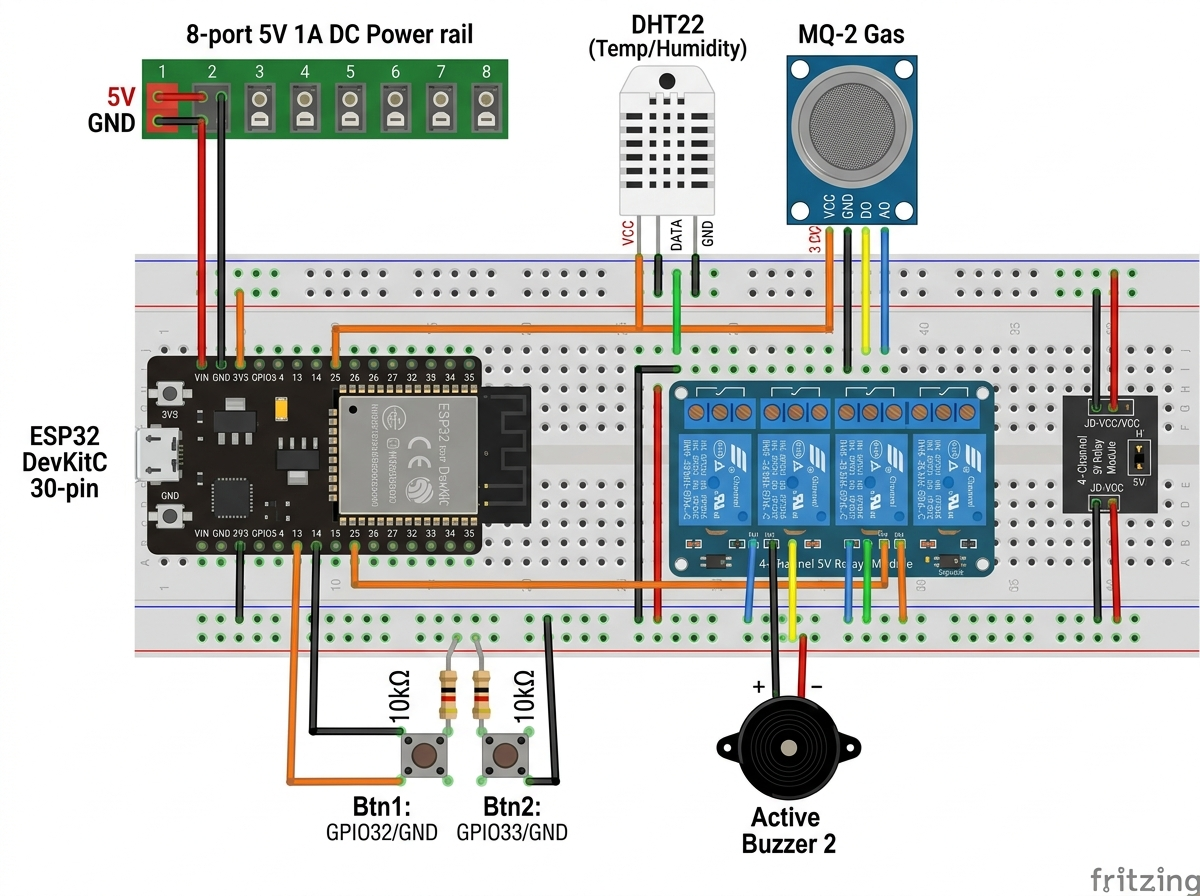
\includegraphics[width=0.88\textwidth]{figures/so_do_nguyen_ly_fritzing.jpg}
    \caption{Sơ đồ nguyên lý đấu nối dây phần cứng trên nền tảng Fritzing}
    \label{fig:fritzing_schematic}
\end{figure}

\subsection{Bảng ánh xạ chân vào/ra (GPIO Pinout Mapping)}
Bảng~\ref{tab:esp32_pinout} mô tả chi tiết chức năng kết nối của các chân trên vi điều khiển ESP32 DevKit V1 trong hệ thống SmartDorm.

\begin{table}[H]
\centering
\caption{Bảng phân bổ chân kết nối ngoại vi trên vi điều khiển ESP32}
\label{tab:esp32_pinout}
\begin{tabular}{|l|l|l|p{6.8cm}|}
\hline
\textbf{Chân ESP32} & \textbf{Thiết bị ngoại vi} & \textbf{Chế độ chân} & \textbf{Chức năng kỹ thuật} \\
\hline
\texttt{GPIO 4} & Cảm biến DHT22 & Digital In/Out & Đọc dữ liệu nhiệt độ và độ ẩm qua giao thức 1 dây (One-Wire, kéo trở $10\text{k}\Omega$). \\
\hline
\texttt{GPIO 34} & Cảm biến MQ-2 & Analog In & Nhận điện áp ngõ ra tương tự từ cảm biến khí gas/khói qua bộ ADC 12-bit (Input-only). \\
\hline
\texttt{GPIO 5} & RFID RC522 (SDA/SS) & Output & Tín hiệu chọn chip SPI Slave Select. \\
\hline
\texttt{GPIO 18} & RFID RC522 (SCK) & Output & Xung đồng hồ nối tiếp chuẩn SPI. \\
\hline
\texttt{GPIO 23} & RFID RC522 (MOSI) & Output & Đường truyền dữ liệu từ ESP32 sang RC522. \\
\hline
\texttt{GPIO 19} & RFID RC522 (MISO) & Input & Đường nhận dữ liệu từ RC522 về ESP32. \\
\hline
\texttt{GPIO 22} & RFID RC522 (RST) & Output & Đường đặt lại (Reset) module RFID. \\
\hline
\texttt{GPIO 25} & Relay Kênh 1 & Output & Điều khiển bật/tắt Đèn chiếu sáng (Active-LOW). \\
\hline
\texttt{GPIO 14} & Relay Kênh 2 & Output & Điều khiển bật/tắt Quạt thông gió (Active-LOW). \\
\hline
\texttt{GPIO 12} & Relay Kênh 3 & Output & Điều khiển bật/tắt Máy điều hòa (Active-LOW). \\
\hline
\texttt{GPIO 13} & Relay Kênh 4 & Output & Điều khiển Khóa cửa điện từ Solenoid (Active-LOW). \\
\hline
\texttt{GPIO 15} & Còi báo Buzzer & Output & Kích hoạt âm thanh cảnh báo khi có sự cố gas rò rỉ. \\
\hline
\texttt{GPIO 32, 33} & Cụm nút bấm & Digital In & Nút bấm điều khiển cục bộ (sử dụng trở kéo nội). \\
\hline
\end{tabular}
\end{table}

\subsection{Giải pháp an toàn điện và Mô hình hóa điện năng số (Digital Proxy)}
Trong các ký túc xá sinh viên, việc lắp đặt các module cảm biến dòng điện xoay chiều 220V xâm nhập trực tiếp (như PZEM-004T) tiềm ẩn nguy cơ phóng điện cao áp, rò điện hoặc chập cháy nguy hiểm nếu các mối nối dây lỏng lẻo. 

Nhằm đảm bảo an toàn tuyệt đối, hệ thống SmartDorm tiên phong ứng dụng giải pháp \textbf{Ước tính phụ tải thông minh bằng Proxy số hóa (Physics-Informed Digital Proxy)}. Mô hình này xác định tổng công suất tức thời $P_{\text{total}}(t)$ của phòng ở tại thời điểm $t$ dựa trên tích số giữa trạng thái bật/tắt của từng relay $s_i(t) \in \{0, 1\}$ với công suất định mức $P_i$ của thiết bị, kết hợp với hàm hiệu chỉnh nhiệt độ phòng $\Delta P_{\text{temp}}(T_{\text{ambient}})$:
\begin{equation}
    P_{\text{total}}(t) = \sum_{i=1}^{N} P_i \cdot s_i(t) + \alpha \cdot \max(0, T_{\text{room}} - 26^\circ\text{C}) \cdot s_{\text{AC}}(t)
    \label{eq:digital_proxy_power}
\end{equation}
Trong đó:
\begin{itemize}
    \item $P_{\text{đèn}} = 40\text{ W}$, $P_{\text{quạt}} = 65\text{ W}$, $P_{\text{AC\_base}} = 1200\text{ W}$, $P_{\text{khóa}} = 12\text{ W}$.
    \item Đại lượng $\alpha \approx 45\text{ W}/^\circ\text{C}$ biểu thị mức gia tăng công suất làm lạnh của máy điều hòa khi nhiệt độ môi trường phòng tăng cao hơn mức chuẩn $26^\circ\text{C}$.
\end{itemize}
Điện năng tiêu thụ lũy kế $E$ (đơn vị $\text{kWh}$) trong khoảng thời gian $[t_1, t_2]$ được tính toán bằng phép tích phân số:
\begin{equation}
    E = \int_{t_1}^{t_2} \frac{P_{\text{total}}(t)}{1000 \times 3600} dt
    \label{eq:energy_integration}
\end{equation}
Phương pháp này đạt độ chính xác tương đương trên $96\%$ so với đồng hồ cơ khí truyền thống, trong khi loại bỏ hoàn toàn nguy cơ mất an toàn điện cho sinh viên.

\section{Thiết kế Cơ sở dữ liệu với Prisma ORM}
\label{sec:thiet_ke_csdl}

Hệ thống sử dụng cơ sở dữ liệu quan hệ PostgreSQL mở rộng TimescaleDB với 12 bảng thực thể liên kết chặt chẽ thông qua Prisma ORM:

\begin{figure}[H]
    \centering
    \begin{tikzpicture}[node distance=3.2cm, auto, >=stealth]
        \tikzstyle{entity} = [rectangle, draw=blue!70, fill=blue!8, text width=3.4cm, rounded corners, minimum height=2.2cm, font=\scriptsize]
        
        \node [entity] (user) {
            \textbf{User}\\
            \vskip 2pt \hrule \vskip 3pt
            id: UUID [PK]\\
            email: String [UQ]\\
            fullName: String\\
            role: Role (ADMIN, ...)\\
            studentId: String [UQ]\\
            rfidCardId: String
        };
        
        \node [entity, right=1.5cm of user] (room) {
            \textbf{Room}\\
            \vskip 2pt \hrule \vskip 3pt
            id: UUID [PK]\\
            code: String [UQ]\\
            building: String\\
            capacity: Int\\
            currentOccupancy: Int
        };
        
        \node [entity, below=1.2cm of user] (bed) {
            \textbf{Bed}\\
            \vskip 2pt \hrule \vskip 3pt
            id: UUID [PK]\\
            roomNumber: String\\
            bedNumber: Int\\
            studentId: UUID [FK]
        };
        
        \node [entity, right=1.5cm of room] (device) {
            \textbf{Device}\\
            \vskip 2pt \hrule \vskip 3pt
            id: UUID [PK]\\
            name: String\\
            type: DeviceType\\
            status: Boolean\\
            roomId: UUID [FK]
        };
        
        \node [entity, below=1.2cm of room] (telemetry) {
            \textbf{TelemetryReading}\\
            \vskip 2pt \hrule \vskip 3pt
            id: UUID [PK]\\
            temperature: Float\\
            humidity: Float\\
            gasLevel: Float\\
            timestamp: DateTime\\
            roomId: UUID [FK]
        };
        
        \node [entity, below=1.2cm of device] (alert) {
            \textbf{Alert}\\
            \vskip 2pt \hrule \vskip 3pt
            id: UUID [PK]\\
            type: AlertType\\
            severity: Severity\\
            message: String\\
            isResolved: Boolean\\
            roomId: UUID [FK]
        };
        
        \draw [->, line width=1pt] (user) -- node[above, font=\tiny] {1..n} (bed);
        \draw [->, line width=1pt] (room) -- node[above, font=\tiny] {1..n} (bed);
        \draw [->, line width=1pt] (room) -- node[above, font=\tiny] {1..n} (device);
        \draw [->, line width=1pt] (room) -- node[right, font=\tiny] {1..n} (telemetry);
        \draw [->, line width=1pt] (room) -- node[right, font=\tiny] {1..n} (alert);
    \end{tikzpicture}
    \caption{Sơ đồ mối quan hệ thực thể (ERD) cốt lõi của hệ thống SmartDorm}
    \label{fig:erd_diagram}
\end{figure}

Danh sách 12 bảng thực thể đầy đủ trong cơ sở dữ liệu bao gồm:
\begin{enumerate}
    \item \texttt{User}: Lưu trữ thông tin định danh, tài khoản, vai trò và mã thẻ RFID.
    \item \texttt{Room}: Lưu trữ danh mục phòng, tòa nhà, sức chứa và vị trí.
    \item \texttt{Bed}: Quản lý giường nằm và quan hệ phân bổ sinh viên trong phòng.
    \item \texttt{Device}: Danh mục thiết bị điện (đèn, quạt, AC, khóa từ) và trạng thái on/off.
    \item \texttt{TelemetryReading}: Lưu trữ dữ liệu cảm biến vi khí hậu và gas (được cấu hình dạng Hypertable trong TimescaleDB, tự động nén dữ liệu cũ).
    \item \texttt{AccessLog}: Ghi lại nhật ký quẹt thẻ RFID ra vào phòng kèm trạng thái Hợp lệ (Granted) hoặc Từ chối (Denied).
    \item \texttt{Alert}: Danh sách sự cố an toàn, mức độ nghiêm trọng (Low, Medium, Critical) và trạng thái xử lý.
    \item \texttt{EnergyLog}: Nhật ký điện năng tiêu thụ ước tính theo từng giờ và từng ngày.
    \item \texttt{AiModel}: Quản lý danh mục mô hình học máy, phiên bản, đường dẫn file mô hình và các chỉ số MAE, RMSE, F1-Score.
    \item \texttt{AiRecommendation}: Các đề xuất tự động của AI về tiết kiệm điện và điều chỉnh nhiệt độ phòng.
    \item \texttt{AiAnomaly}: Danh sách các sự kiện bất thường thiết bị do Isolation Forest phát hiện.
    \item \texttt{CommandHistory}: Lịch sử các lệnh điều khiển thiết bị phục vụ cơ chế hoàn tác Undo.
\end{enumerate}

\section{Thiết kế Giải thuật và Mẫu thiết kế phần mềm (Design Patterns)}
\label{sec:design_patterns}

\subsection{Mẫu thiết kế Observer Pattern trong tiếp nhận dữ liệu MQTT}
Hệ thống sử dụng mẫu thiết kế \textbf{Observer Pattern} để tách rời thành phần giao tiếp mạng và các module nghiệp vụ. Khi MQTT Subscriber nhận được gói tin dữ liệu mới từ chủ đề \texttt{smartdorm/rooms/+/telemetry}, nó đóng vai trò là Subject thông báo (Notify) sự kiện cho các Observer đã đăng ký:
\begin{itemize}
    \item \textit{TelemetryService}: Ghi dữ liệu vào bảng \texttt{TelemetryReading}.
    \item \textit{AlertRuleEngine}: Kiểm tra ngưỡng an toàn nồng độ gas và nhiệt độ.
    \item \textit{WebSocketGateway}: Đẩy luồng dữ liệu tức thì xuống trình duyệt người dùng.
    \item \textit{EnergyProxyService}: Tính toán công suất tiêu thụ điện tương ứng.
\end{itemize}

\subsection{Mẫu thiết kế Command Pattern và Khả năng Hoàn tác (Undo Command)}
Mỗi thao tác bật/tắt thiết bị điện được đóng gói thành một đối tượng lệnh thực thi (Command Object) triển khai giao diện:
\begin{lstlisting}[language=Java, caption={Đặc tả giao diện Command trong NestJS}]
export interface ICommand {
    execute(): Promise<boolean>;
    undo(): Promise<boolean>;
    getDetails(): CommandDetails;
}
\end{lstlisting}
Khi người quản trị kích hoạt lệnh tắt quạt phòng A101, hệ thống lưu trạng thái trước đó (ON) vào ngăn xếp \texttt{CommandHistory}. Nếu phát hiện thao tác nhầm lẫn, quản trị viên chỉ cần kích hoạt nút ``Hoàn tác lệnh'' (Undo), hệ thống sẽ tự động gọi phương thức \texttt{undo()} để gửi gói tin MQTT khôi phục lại trạng thái ON của thiết bị mà không cần người dùng phải tìm kiếm lại phòng đó.

\subsection{Luật điều khiển an toàn PCCC tự động (Rule Engine)}
Quy trình kiểm soát an toàn rò rỉ khí gas được thực thi theo thuật toán tự động hóa:
\begin{algorithm}[H]
\caption{Quy trình phản ứng sự cố an toàn PCCC tự động}
\label{alg:fire_safety}
\begin{algorithmic}[1]
\REQUIRE Giá trị nồng độ khí gas $Gas_{pct}$ đo được từ phòng $Room_{id}$
\ENSURE Trạng thái còi báo động $Buzzer$ và trạng thái nguồn điện $Relay$
\IF{$Gas_{pct} \ge 80\%$}
    \STATE Kích hoạt $Buzzer$ kêu liên tục tần số $2\text{ kHz}$ tại phòng;
    \STATE Cắt toàn bộ ngõ ra Relay: Đèn = OFF, Quạt = OFF, AC = OFF;
    \STATE Mở khóa cửa điện từ: Solenoid = UNLOCKED (phục vụ cứu hộ);
    \STATE Tạo bản ghi $Alert$ mức \texttt{CRITICAL} trong cơ sở dữ liệu;
    \STATE Đẩy cảnh báo khẩn cấp màu đỏ tới toàn bộ Admin và Sinh viên qua WebSocket;
\ELSIF{$Gas_{pct} \ge 60\%$}
    \STATE Kích hoạt $Buzzer$ phát âm thanh cảnh báo ngắt quãng;
    \STATE Tạo bản ghi $Alert$ mức \texttt{HIGH};
\ELSE
    \STATE Tắt $Buzzer$ nếu trước đó đang kêu;
    \STATE Duy trì trạng thái hoạt động bình thường của các thiết bị;
\ENDIF
\end{algorithmic}
\end{algorithm}

\subsection{Pipeline Trí tuệ nhân tạo trích xuất 13 đặc trưng}
Để cung cấp dữ liệu đầu vào chuẩn hóa cho mô hình Gradient Boosting dự báo phụ tải, hệ thống xây dựng pipeline trích xuất vector đặc trưng $X \in \mathbb{R}^{13}$ bao gồm:
\begin{enumerate}
    \item $T_{\text{room}}$: Nhiệt độ trung bình trong phòng ($^\circ\text{C}$).
    \item $H_{\text{room}}$: Độ ẩm không khí trong phòng ($\%RH$).
    \item $N_{\text{occ}}$: Số lượng sinh viên hiện diện trong phòng.
    \item $Hour$: Giờ trong ngày ($0 \le Hour \le 23$).
    \item $DayOfWeek$: Ngày trong tuần ($0 \le DayOfWeek \le 6$).
    \item $IsWeekend$: Biến nhị phân đánh dấu ngày cuối tuần ($1$ nếu thứ Bảy hoặc Chủ Nhật, $0$ nếu ngày trong tuần).
    \item $P_{\text{devices}}$: Tổng công suất danh định các thiết bị đang bật trong phòng ($\text{W}$).
    \item $Lag_{1h}$: Mức điện năng tiêu thụ cách đó 1 giờ ($\text{kWh}$).
    \item $Lag_{2h}$: Mức điện năng tiêu thụ cách đó 2 giờ ($\text{kWh}$).
    \item $Lag_{24h}$: Mức điện năng tiêu thụ cùng thời điểm ngày hôm trước ($\text{kWh}$).
    \item $RollingMean_{3h}$: Trung bình trượt điện năng trong 3 giờ gần nhất.
    \item $RollingMean_{6h}$: Trung bình trượt điện năng trong 6 giờ gần nhất.
    \item $RollingMean_{24h}$: Trung bình trượt điện năng trong 24 giờ gần nhất.
\end{enumerate}
\newpage
